%% Excised material from "Who does the new work?" -- archive memo.
%% Not for publication now; kept verbatim for future use. Each block
%% carries its provenance and the reason it failed the deletion test
%% (no result becomes unreportable or undefendable without it).
%% Revival: paste back and restore the cross-reference stitches listed
%% in patch 11; the notation rows at the end belong to the wedge and
%% demand blocks.

%% ==================================================================
%% EXCISED: Sec. 3.3 Assignment interpretation
%% Source: paper/who_does_the_new_work.tex, lines 527-551 (pre-excision commit)
%% Reason: duplicates the assignment-programme appendix; interpretive, not result-bearing
%% ==================================================================

\subsection{Assignment interpretation}
\label{sec:assignment-interpretation}

The field $\Pi(\mathbf{r})$ is used as a fixed reduced form in the main
model, but it is not atheoretic. Appendix~\ref{app:assignment}
interprets it as the price surface of a multidimensional assignment
equilibrium in the sense of \textcite{lindenlaub2017}: occupations are
capability types, task demand is CES over locations, and no observed
wage enters the computation, so agreement with the estimated field is a
test rather than a fit. Uniform demand recovers the field's shape (rank
correlation $+0.92$) but not its directed gradient; a single cognitive
demand shifter recovers both ($+0.97$, gradient $+0.36$ against the
estimated $+0.39$). The dearness of cognitive work reads as
demand-driven assignment pressure rather than productivity superiority.

The exercise supports the reduced form; the main results do not need
it. The comparative statics below hold the surface fixed, and
re-solving the assignment after a technology shock is a
general-equilibrium extension expected to dampen, not reverse, the
mechanisms studied here. The appendix also states the exercise's scope:
it reproduces the field's shape, not the observed concentration of
employment.


%% ============================================================

%% ==================================================================
%% EXCISED: Sec. 4.2 Cost saving and the second-order margin
%% Source: paper/who_does_the_new_work.tex, lines 667-699 (pre-excision commit)
%% Reason: technical qualification; no result consumes it
%% ==================================================================

\subsection{Cost saving and the second-order margin}
\label{sec:cost-saving}

Where capital bears the operated share, unit cost falls from
$\Pi(\mathbf{r})$ to
\begin{equation}
  c(\mathbf{r})
  =
  (1-a(\mathbf{r}))\Pi(\mathbf{r})
  +
  a(\mathbf{r})
  \frac{R}{s_K\phi_K(\mathbf{r})}.
  \label{eq:unit-cost}
\end{equation}
The realized per-unit saving is
\[
  \Pi(\mathbf{r}) - c(\mathbf{r})
  =
  a(\mathbf{r})
  \left[
    \Pi(\mathbf{r})
    -
    \frac{R}{s_K\phi_K(\mathbf{r})}
  \right].
\]
This saving is largest deep inside the technology's core, where capital
has a strong cost advantage. It vanishes at the adoption margin, because
the marginal task capital just takes is one it produces at approximately
the same cost as labour. This second-order margin is central to the
employment results below. Displacement begins as soon as the operated
share rises, but the demand channel is weak until infra-marginal savings
are large.


%% ==================================================================
%% EXCISED: Sec. 4.5 The bundle operator
%% Source: paper/who_does_the_new_work.tex, lines 839-886 (pre-excision commit)
%% Reason: operator formalism; results use the constructions, not the algebra
%% ==================================================================

\subsection{The bundle operator}
\label{sec:bundle-operator}

The post-technology bundle is
\begin{equation}
  b_o^{\text{post}}(\mathbf{r})
  =
  b_o(\mathbf{r})(1-a(\mathbf{r}))
  +
  \frac{\iota_o(\mathbf{r})}{L_o}.
  \label{eq:bundle-operator}
\end{equation}
The occupation is therefore not abolished. Its paid task content is
redrawn. Automation strips operated content; reinstatement adds bound
seeded content.

The operator does not preserve bundle mass. Its integral is
\[
  \int b_o^{\text{post}}(\mathbf{r})\,d\mathbf{r}
  =
  1 - D_o + B_o/L_o,
\]
where $B_o=\int\iota_o(\mathbf{r})\,d\mathbf{r}$. We do not renormalize
the bundle, because doing so would assume that freed time is
proportionally reallocated across remaining tasks. In this model, the
mass deficit is exactly the labour released to the worker-sorting
layer.

The wage change implied by bundle rewriting is
\begin{equation}
  \Delta w_o
  =
  \int
  \Pi(\mathbf{r})
  \left[
    -b_o(\mathbf{r})a(\mathbf{r})
    +
    \frac{\iota_o(\mathbf{r})}{L_o}
  \right]
  d\mathbf{r}.
  \label{eq:wage-change}
\end{equation}
The first term removes paid content, typically from high-priced tasks.
The second term adds new human task content, but only where the deficit
gate permits attachment. Reinstatement therefore carries a downward
wage bias when it strips high-priced work and refills with lower-priced
work.


%% ==================================================================
%% EXCISED: Sec. 6.4 Family wage wedge (gate weights retained in the paper)
%% Source: paper/who_does_the_new_work.tex, lines ~1289-1311 (pre-excision commit)
%% Reason: robustness layer on the adoption margin; mechanism reported without it
%% ==================================================================

The residual wage wedge is
\[
  \omega_o
  =
  \ln w_{\text{obs},o}
  -
  \ln w_{\text{bundle},o}.
\]
The family wedge $\omega_g$ is the family-level mean of this residual.
It is measured once and held fixed under technology shocks. When used,
it enters the adoption gate through
\[
  \Pi_{\text{eff}}=e^{\omega_g}\Pi.
\]
The main mechanism is reported with and without this wedge
(Figure~\ref{fig:family-wedge-new}).

\begin{figure}[!htbp]
\centering
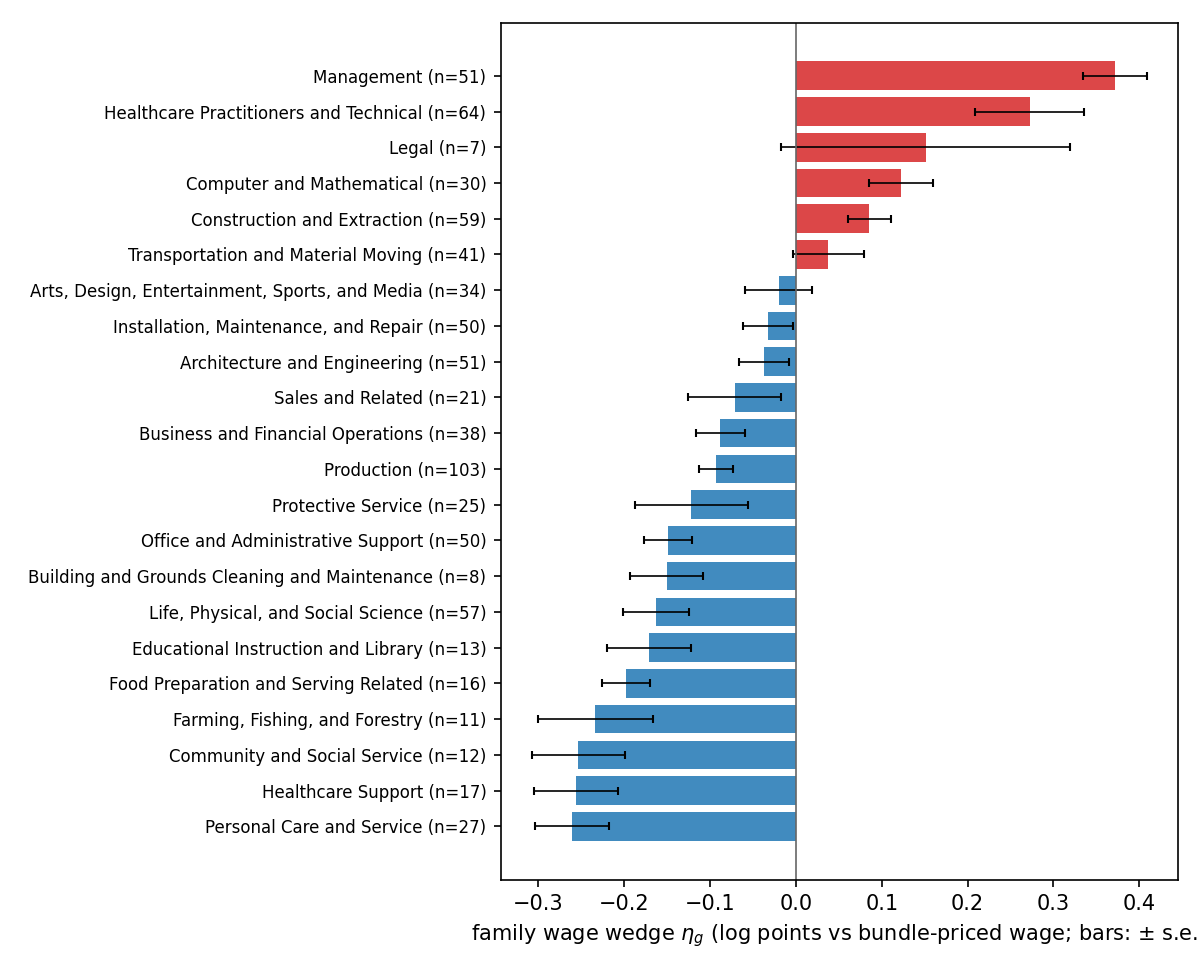
\includegraphics[width=0.8\textwidth]{family_wedge.png}
\caption{Family wage wedge $\omega_g$: mean log deviation of observed wages from the bundle-priced wage, by job family. Management sits highest above the field and Personal Care and Service lowest below it; the wedge enters only the adoption margin.}
\label{fig:family-wedge-new}
\end{figure}



%% ==================================================================
%% EXCISED: Sec. 6.6 Automation waves as technology fields
%% Source: paper/who_does_the_new_work.tex, lines 1402-1486 (pre-excision commit)
%% Reason: expressiveness display, not result-bearing; the robot-field calibration it carried migrated to sec:robot-field
%% ==================================================================

\subsection{Automation waves as technology fields}
\label{sec:automation-waves}

The same calibration locates other technologies. \textcite{webb2020}
builds occupational exposure to three technologies by matching patent
text to O*NET tasks: industrial robots, software, and machine learning.
Fitting each to the disk, beside the language-model exposure, places
four technologies in one geometry (Table~\ref{tab:webb-fields},
Figure~\ref{fig:webb-fields}). Webb's measures are occupation-level, so
all four are fitted on the occupation substrate here; the cognitive
field's centre reported below ($40^\circ$) is its occupation-substrate
fit, while the analysis uses its task-level calibration of
Table~\ref{tab:technology-calibration-new}.

Read in the order the technologies diffused, the fields sweep across the
space. Industrial robots sit in the technical-physical west, at the
periphery where production and manual work lie, with a narrow reach.
Software sits to the north-west, over routine technical work. Machine
learning, the AI of Webb's patents through about 2018, sits in the
analytical north. Language models sit in the north-east, broad over
high-priced cognitive work. The centres fall in an arc from the physical
west to the cognitive north-east, in the order the waves arrived. This
is the spatial form of the succession of automation technologies
documented by \textcite{acemoglu2020robots} for robots and by
\textcite{autor2003} for computerisation: each wave acts on different
work, and the geometry locates where.

Two of the four fields are localised. The robot field and the
language-model field centre inside the occupied disk, and their reach
follows a concentrated exposure. The robot field is narrow and western;
the language-model field is broad and north-east. The software and
machine-learning surfaces are gradients rather than peaks. Exposure
rises toward the north without an interior maximum, so a single field
centres at the edge of the occupied region and its reach is an artefact
of that shape. Webb's machine learning locates AI further north than the
language-model measure and does not coincide with it, which is expected,
since patent-era machine learning and language models are different
technologies acting on different work.

Three limits bound the reading. The chronology is external to the data.
Webb's three measures are built from patents through about 2018, so they
do not date the technologies; the order comes from when each diffused.
The measures do not share a source, since robots, software, and machine
learning are one construction and language models another. And four
fields illustrate the mechanism, not a temporal law. Within those limits
the figure does what the representation is for: it places several
technologies in one geometry according to where each acts.

\begin{table}[!htbp]
\centering
\caption{The four technology fields fitted on the common occupation
substrate, in the order the technologies diffused. Robots, software, and
machine learning are the patent-based exposures of \textcite{webb2020};
language models are the LLM exposure of \textcite{eloundou2024}. Fit is
the $R^2$ on the between-cell exposure surface; the centre column marks
fields whose centre sits at the edge of the occupied disk (support
$\chi=0.75$). The cognitive field's analysis calibration is the
task-level fit of Table~\ref{tab:technology-calibration-new}.}
\label{tab:webb-fields}
\begin{tabular}{llccccl}
\toprule
Technology & Source & $\xi_K$ & $\chi_K$ & $z_K$ & $R^2$ & Centre \\
\midrule
Industrial robots & Webb      & $207^\circ$ & $0.75$ & $0.50$ & $0.84$ & at edge \\
Software          & Webb      & $146^\circ$ & $0.75$ & $0.80$ & $0.62$ & at edge \\
Machine learning  & Webb      & $108^\circ$ & $0.75$ & $0.70$ & $0.70$ & at edge \\
Language models   & Eloundou  & $40^\circ$  & $0.49$ & $0.57$ & $0.83$ & localised \\
\bottomrule
\end{tabular}
\end{table}

\begin{figure}[!htbp]
\centering
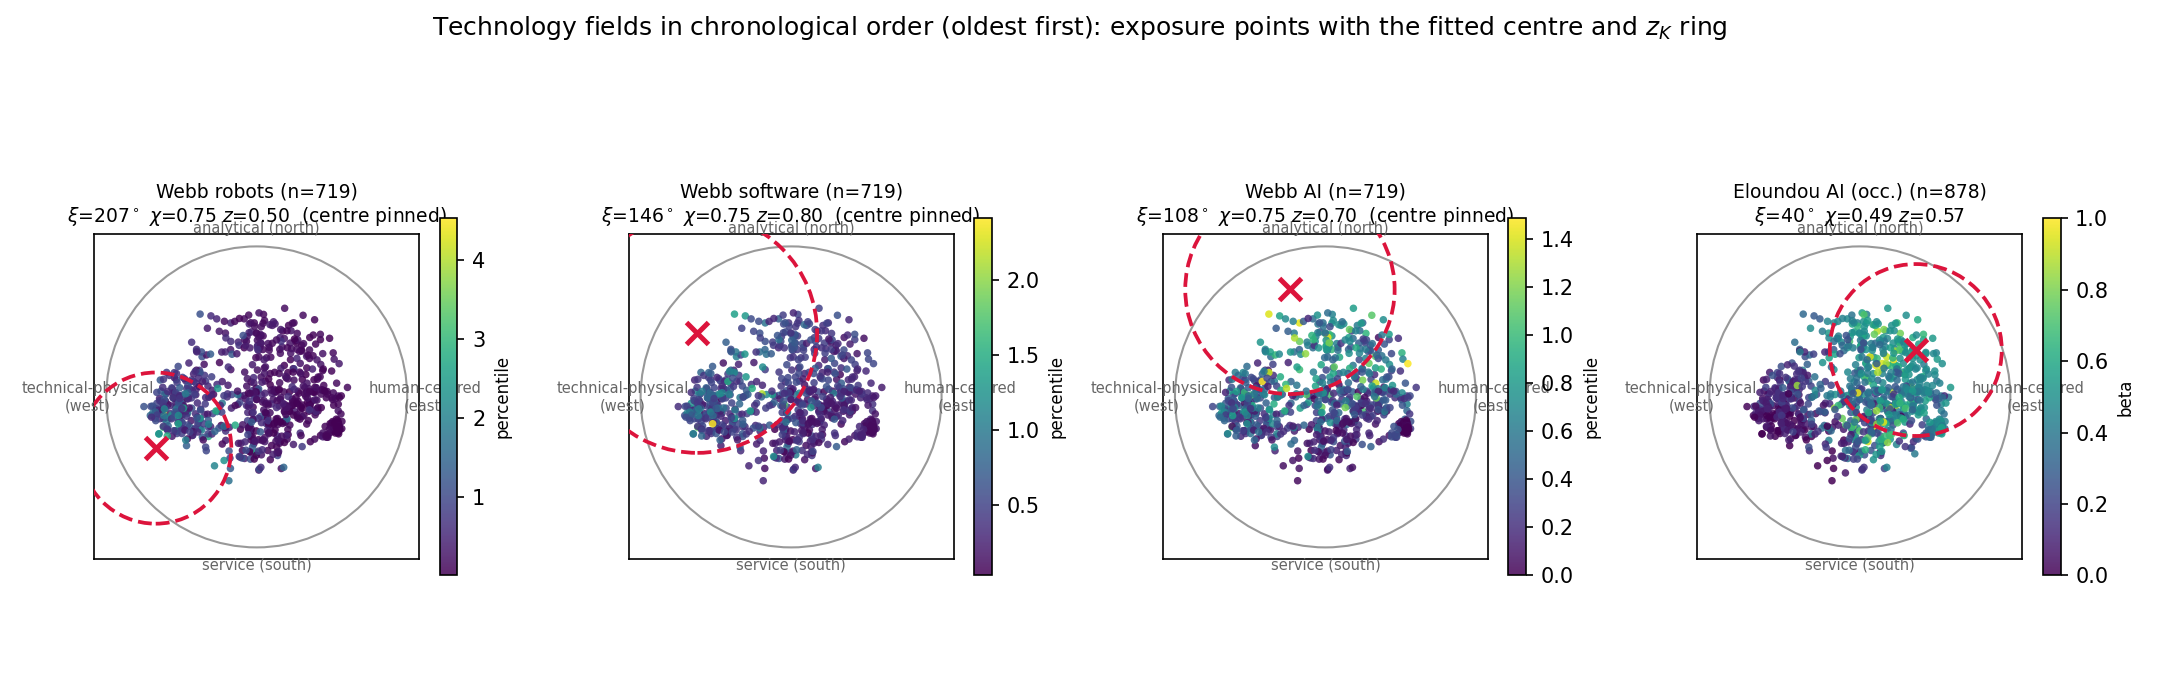
\includegraphics[width=\textwidth]{webb_points_and_rings.png}
\caption{The four technology fields, oldest first. Each panel shows the
occupations coloured by their exposure to one technology, with the
fitted field centre ($\times$) and the $z_K$ ring. Industrial robots,
software, and machine learning are from \textcite{webb2020}; language
models from \textcite{eloundou2024}. The robot and language-model fields
enclose a concentrated exposure; the software and machine-learning
surfaces rise toward the north without an interior peak, so their fitted
centre sits at the edge of the occupied disk.}
\label{fig:webb-fields}
\end{figure}


%% ==================================================================
%% EXCISED: Sec. 7.3 The demand channel
%% Source: paper/who_does_the_new_work.tex, lines 1716-1749 (pre-excision commit)
%% Reason: sensitivity analysis; eta layer not consumed by the headline results
%% ==================================================================

\subsection{The demand channel}
\label{sec:case-demand}

The demand channel is evaluated by sweeping the output-demand elasticity
$\eta$. At unit-elastic demand, cost savings leave revenue unchanged.
Both technology fields release labour in their automated region, by
$12$ percent for the cognitive field and $22$ percent for the robot one
(Figure~\ref{fig:demand-new}).
Across plausible elasticities, displacement dominates because savings
are small at the adoption margin: the price-to-cost ratio is essentially
one there against roughly $1.5$ deep in the cognitive core and $1.2$ in
the robot core. Net
employment growth requires elasticity beyond the plausible range: the
cognitive region crosses zero at $\eta\approx8$, and the robot region
does not cross below $\eta=12$, because its core saving is smaller and
the demand channel has less to hand back.

\begin{figure}[!htbp]
\centering
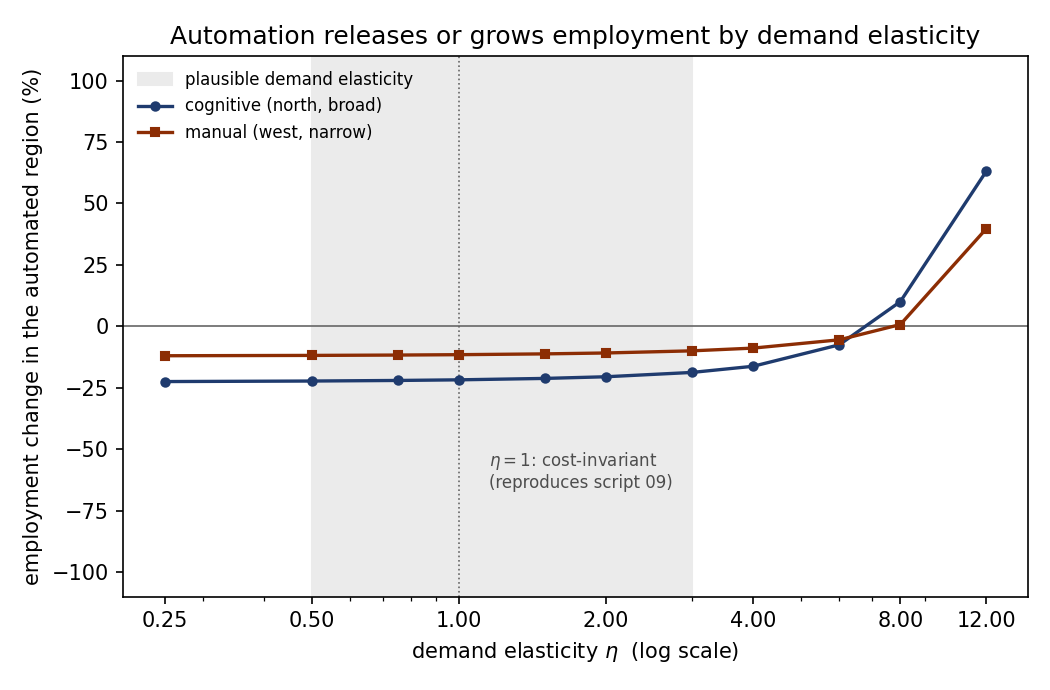
\includegraphics[width=0.85\textwidth]{demand_channel_eta.png}
\caption{Employment change in each technology field's automated region
as a function of output-demand elasticity.}
\label{fig:demand-new}
\end{figure}

This recovers the contrast emphasized by \textcite{bessen2019demand}.
Automation in an inelastic-demand direction releases labour; automation
in an elastic-demand direction can draw labour in. The disk adds the
location. Mechanised agriculture and nineteenth-century
textiles occupy different places on the elasticity scale; cognitive
automation is conditional on the still uncertain elasticity of demand
for cognitive output.

%% ============================================================

%% ==================================================================
%% EXCISED: Notation rows (wedge and demand)
%% Source: paper/who_does_the_new_work.tex, lines ~2419-2421 (pre-excision commit)
%% Reason: belong to the excised wedge and demand blocks
%% ==================================================================

$\omega_o=\ln w_{\mathrm{obs},o}-\ln w_{\mathrm{bundle},o}$ & occupation rent (residual of log wage on priced content) \\
$\omega_g$ & family wage wedge: the family mean of $\omega_o$ \\
$\eta$ & demand elasticity (Section~\ref{sec:case-demand}) \\
